I test di unità servono ad assicurare il funzionamento delle più piccole unità software, ovvero i singoli metodi, indipendentemente dal sistema in cui sono presenti.

\subsubsection{Test di unità previsti}

\begin{tabularx}{\textwidth}{cXc}
	
	\rowcolor{greySWEight}
	
	\rowcolor{greySWEight}
	\textcolor{white}{\textbf{Codice}} & 
	\textcolor{white}{\textbf{Descrizione}} &
	\textcolor{white}{\textbf{Stato}} \\
	
	\textbf{TU001} & Verifica che il flag di attivazione utente sia messo a true correttamente & \textcolor{ForestGreen}{Superato} \\
	\textbf{TU002} & Verifica che il metodo ritorni tutti gli utenti presenti nel sistema & \textcolor{ForestGreen}{Superato} \\
	\textbf{TU003} & Verifica che il metodo ritorni tutte le frasi in cui uno specifico utente ha inserito almeno una soluzione & \textcolor{ForestGreen}{Superato} \\
	\textbf{TU004} & Verifica che il metodo ritorni tutte le soluzioni inserite da uno specifico utente & \textcolor{ForestGreen}{Superato} \\
	\textbf{TU005} & Verifica che l'affidabilità di una soluzione venga incrementata correttamente & \textcolor{ForestGreen}{Superato} \\
	\textbf{TU006} & Verifica che il metodo ritorni una specifica soluzione dato il suo ID & Non Implementato \\
	\textbf{TU007} & Verifica che il nome dell'autore dell'esercizio venga modificato correttamente & \textcolor{ForestGreen}{Superato} \\
	\textbf{TU008} & Verifica che un utente venga inserito correttamente nel sistema & \textcolor{ForestGreen}{Superato} \\
	\textbf{TU009} & Verifica che il metodo ritorni l'utente corretto dato il suo ID & \textcolor{ForestGreen}{Superato} \\
	\textbf{TU010} & Verifica che il metodo ritorni l'utente corretto dato il suo ID oppure un'eccezione se non è presente nel sistema & \textcolor{ForestGreen}{Superato} \\
	\textbf{TU011} & Verifica che un utente venga attivato correttamente & \textcolor{ForestGreen}{Superato} \\
	\textbf{TU012} & Verifica che un utente venga cancellato correttamente & \textcolor{ForestGreen}{Superato} \\
	\textbf{TU013} & Verifica che il metodo ritorni l'utente corretto data l'email di iscrizione & \textcolor{ForestGreen}{Superato} \\
	\textbf{TU014} & Verifica che il metodo aggiorni correttamente i dati di uno specifico utente & \textcolor{ForestGreen}{Superato} \\
	\textbf{TU015} & Verifica che il metodo assegni correttamente un esercizio a uno o più utenti & \textcolor{ForestGreen}{Superato} \\
	\textbf{TU016} & Verifica che il metodo ritorni tutti gli esercizi assegnati ad un utente & \textcolor{ForestGreen}{Superato} \\
	\textbf{TU017} & Verifica che il metodo ritorni tutti gli allievi presenti nel sistema & \textcolor{ForestGreen}{Superato} \\
	\textbf{TU018} & Verifica che il metodo ritorni tutti gli utenti presenti nel sistema & \textcolor{ForestGreen}{Superato} \\
	\textbf{TU019} & Verifica che il metodo rimuova un esercizio dalla lista di esercizi assegnati ad utente & \textcolor{ForestGreen}{Superato} \\
	\textbf{TU020} & Verifica che il metodo ritorni tutti gli esercizi svolti da un utente & \textcolor{ForestGreen}{Superato} \\
	\textbf{TU021} & Verifica che un esercizio venga aggiunto alla lista di esercizi svolti da un utente & \textcolor{ForestGreen}{Superato} \\
	\textbf{TU022} & Verifica che il metodo ritorni tutti gli sviluppatori non ancora attivati & \textcolor{ForestGreen}{Superato} \\
	\textbf{TU023} & Verifica che il metodo ritorni la soluzione automatica generata da FreeLing & Non Implementato \\
	\textbf{TU024} & Verifica che la frase venga inserita correttamente nel sistema & \textcolor{ForestGreen}{Superato} \\
	\textbf{TU025} & Verifica che il metodo ritorni la frase corretta dato il suo ID & \textcolor{ForestGreen}{Superato} \\
	\textbf{TU026} & Verifica che l'affidabilità di una soluzione venga incrementata correttamente & \textcolor{ForestGreen}{Superato} \\
	\textbf{TU027} & Verifica che il metodo ritorni una specifica soluzione dato il suo ID & \textcolor{ForestGreen}{Superato} \\
	\textbf{TU028} & Verifica che il nome dell'autore dell'esercizio venga modificato correttamente & \textcolor{ForestGreen}{Superato} \\
	\textbf{TU029} & Verifica che l'esercizio venga inserito correttamente nel sistema & \textcolor{ForestGreen}{Superato} \\
	\textbf{TU030} & Verifica che la soluzione di un esercizio proposta da un allievo venga valutata e inserita correttamente & \textcolor{ForestGreen}{Superato} \\
	\textbf{TU031} & Verifica che la soluzione inserita da un allievo venga valutata correttamente & \textcolor{ForestGreen}{Superato} \\
	\textbf{TU032} & Verifica che un esercizio venga cancellato correttamente & \textcolor{ForestGreen}{Superato} \\
	\textbf{TU033} & Verifica che il metodo ritorni tutti gli esercizi richiesti data una lista di ID & \textcolor{ForestGreen}{Superato} \\
	\textbf{TU034} & Verifica che uno specifico utente venga cancellato correttamente & \textcolor{ForestGreen}{Superato} \\
	\textbf{TU035} & Verifica che il metodo ritorni tutti gli sviluppatori non ancora attivati & \textcolor{ForestGreen}{Superato} \\
	\textbf{TU036} & Verifica che il metodo ritorni tutti gli utenti presenti nel sistema & \textcolor{ForestGreen}{Superato} \\
	\textbf{TU037} & Verifica che il metodo effettui il login nel sistema correttamente & Non Implementato \\
	\textbf{TU038} & Verifica che il metodo ritorni l'utente corretto dato il suo ID & \textcolor{ForestGreen}{Superato} \\
	\textbf{TU039} & Verifica che il metodo modifichi correttamente il nome dell'autore di un esercizio & \textcolor{ForestGreen}{Superato} \\
	\textbf{TU040} & Verifica che un utente venga attivato correttamente & \textcolor{ForestGreen}{Superato} \\
	\textbf{TU041} & Verifica che un esercizio venga inserito correttamente & \textcolor{ForestGreen}{Superato} \\
	\textbf{TU042} & Verifica che un esercizio venga svolto e valutato correttamente & \textcolor{ForestGreen}{Superato} \\
	\textbf{TU043} & Verifica che il metodo ritorni la soluzione automatica generata da FreeLing & \textcolor{ForestGreen}{Superato} \\
	\textbf{TU044} & Verifica che il metodo ritorni gli esercizi assegnati a un utente & \textcolor{ForestGreen}{Superato} \\
	\textbf{TU045} & Verifica che il metodo ritorni gli esercizi svolti da un utente & \textcolor{ForestGreen}{Superato} \\
	\textbf{TU046} & Verifica che il metodo ritorni la lista di tutti gli allievi presenti nel sistema & \textcolor{ForestGreen}{Superato} \\
	\textbf{TU047} & Verifica che per utente Studente venga renderizzata sidebarElementStudent & \textcolor{ForestGreen}{Superato} \\
	\textbf{TU048} & Verifica che per utente Insegnante venga renderizzata la sidebarElementTeacher & \textcolor{ForestGreen}{Superato} \\
	\textbf{TU049} & Verifica che per utente Amministratore venga renderizzata sidebarElementAmministrator & \textcolor{ForestGreen}{Superato} \\
	\textbf{TU050} & Verifica che per utente Sviluppatore venga renderizzata sidebarElementDeveloper & \textcolor{ForestGreen}{Superato} \\
	\textbf{TU051} & Verifica che per ogni frase inserita con n parole vengano generate n serie di pulsanti & \textcolor{ForestGreen}{Superato} \\
	\textbf{TU052} & Verifica che ad ogni chiamata del metodo \_translator non ritorni mai un valore nullo. & \textcolor{ForestGreen}{Superato} \\
	\textbf{TU053} & Verifica che il componente ExecutionExercise venga renderizzato passandogli come props qualsiasi
	frase & \textcolor{ForestGreen}{Superato} \\
	\textbf{TU054} & Verifica che il metodo getCodeSolution() della classe SolutionMapper ritorni un valore diverso da NULL & \textcolor{ForestGreen}{Superato} \\
	\textbf{TU055} & Verifica che il metodo getVerboseSolution() della classe SolutionMapper ritorni un valore diverso da NULL & \textcolor{ForestGreen}{Superato} \\
	\textbf{TU056} & Verifica che il metodo getSolution() della classe SolutionMapper ritorni un valore diverso da NULL & \textcolor{ForestGreen}{Superato} \\
	\textbf{TU057} & Verifica che il metodo getCodeSolution del file languageIterator ritorni una frase contentente 
	lo stesso numero di parole e punteggiatura contenuto nella frase di ingresso  & \textcolor{ForestGreen}{Superato} \\
	\textbf{TU058} & Verifica che ad ogni chiamata del metodo \_translator non ritorni mai una stringa. & \textcolor{ForestGreen}{Superato} \\
	\textbf{TU059} & Verifica che in AdminDevDashBoard la variabile auth nello store sia abbia sempre ROLE ADMINISTRATOR & \textcolor{ForestGreen}{Superato} \\
	\textbf{TU060} & Verifica che in AdminUserDashBoard la variabile auth nello store sia valorizzata & \textcolor{ForestGreen}{Superato} \\
	\textbf{TU061} & Verifica che in Dashboard la variabile auth nello store sia valorizzata & \textcolor{ForestGreen}{Superato} \\
	\textbf{TU062} & Verifica che in DeveloperDashBoard la variabile auth nello store sia valorizzata & \textcolor{ForestGreen}{Superato} \\
	\textbf{TU063} & Verifica che in DoneHomework la variabile auth nello store sia valorizzata & \textcolor{ForestGreen}{Superato} \\
	\textbf{TU064} & Verifica che in Homework la variabile auth nello store sia valorizzata & \textcolor{ForestGreen}{Superato} \\
	\textbf{TU065} & Verifica che in HomeworkExecution la variabile auth nello store sia valorizzata & \textcolor{ForestGreen}{Superato} \\
	\textbf{TU066} & Verifica che in InsertExercise la variabile auth nello store sia valorizzata & \textcolor{ForestGreen}{Superato} \\
	\textbf{TU067} & Verifica che in NewExercise la variabile auth nello store sia valorizzata & \textcolor{ForestGreen}{Superato} \\
	\textbf{TU068} & Verifica che in PublicExercise la variabile auth nello store sia valorizzata & \textcolor{ForestGreen}{Superato} \\
	\textbf{TU069} & Verifica che in Navbar la variabile auth nello store sia valorizzata & \textcolor{ForestGreen}{Superato} \\
	\textbf{TU070} & Verifica che authReducer ritorni il nuovo state corretto applicando action: INIT\_AUTH\_STORE & \textcolor{ForestGreen}{Superato} \\
	\textbf{TU071} & Verifica che authReducer ritorni il nuovo state corretto applicando action: CHANGE\_SIGNIN\_DATA & \textcolor{ForestGreen}{Superato} \\
	\textbf{TU072} & Verifica che authReducer ritorni il nuovo state corretto applicando action: CHANGE\_SIGNUP\_DATA & \textcolor{ForestGreen}{Superato} \\
	\textbf{TU037} & Verifica che authReducer ritorni il nuovo state corretto applicando action: LOADER\_ON & \textcolor{ForestGreen}{Superato} \\
	\textbf{TU074} & Verifica che authReducer ritorni il nuovo state corretto applicando action: LOAD\_AUTH & \textcolor{ForestGreen}{Superato} \\
	\textbf{TU075} & Verifica che authReducer ritorni il nuovo state corretto applicando action: LOGIN\_ERROR & \textcolor{ForestGreen}{Superato} \\
	\textbf{TU076} & Verifica che authReducer ritorni il nuovo state corretto applicando action: LOGIN\_SUCCESS & \textcolor{ForestGreen}{Superato} \\
	\textbf{TU077} & Verifica che authReducer ritorni il nuovo state corretto applicando action: SIGNOUT\_SUCCESS & \textcolor{ForestGreen}{Superato} \\
	\textbf{TU078} & Verifica che authReducer ritorni il nuovo state corretto applicando action: SIGNUP\_ERROR & \textcolor{ForestGreen}{Superato} \\
	\textbf{TU079} & Verifica che authReducer ritorni il nuovo state corretto applicando action: SIGNUP\_SUCCESS & \textcolor{ForestGreen}{Superato} \\
	\textbf{TU080} & Verifica che authReducer ritorni il nuovo state corretto applicando action: DISPLAY\_ERROR & \textcolor{ForestGreen}{Superato} \\
	\textbf{TU081} & Verifica che adminReducer ritorni il nuovo state corretto applicando action: INIT\_STATE & non implementato \\
	\textbf{TU082} & Verifica che adminReducer ritorni il nuovo state corretto applicando action: UPDATE\_FILTER & \textcolor{ForestGreen}{Superato} \\
	\textbf{TU083} & Verifica che adminReducer ritorni il nuovo state corretto applicando action: UPDATE\_DEV\_LIST & \textcolor{ForestGreen}{Superato} \\
	\textbf{TU084} & Verifica che adminReducer ritorni il nuovo state corretto applicando action: UPDATE\_USER\_LIST & \textcolor{ForestGreen}{Superato} \\
	\textbf{TU085} & Verifica che adminReducer ritorni il nuovo state corretto applicando action: USER\_DELETE\_SUCCES & \textcolor{ForestGreen}{Superato} \\
	\textbf{TU086} & Verifica che adminReducer ritorni il nuovo state corretto applicando action: DEV\_APPROVE\_SUCCES & \textcolor{ForestGreen}{Superato} \\
	
	
	\rowcolor{white}
	\caption{Test di unità}
	\label{tab:tabellatestunità}
\end{tabularx}

% \begin{figure}[H]
% 	\centering
% 	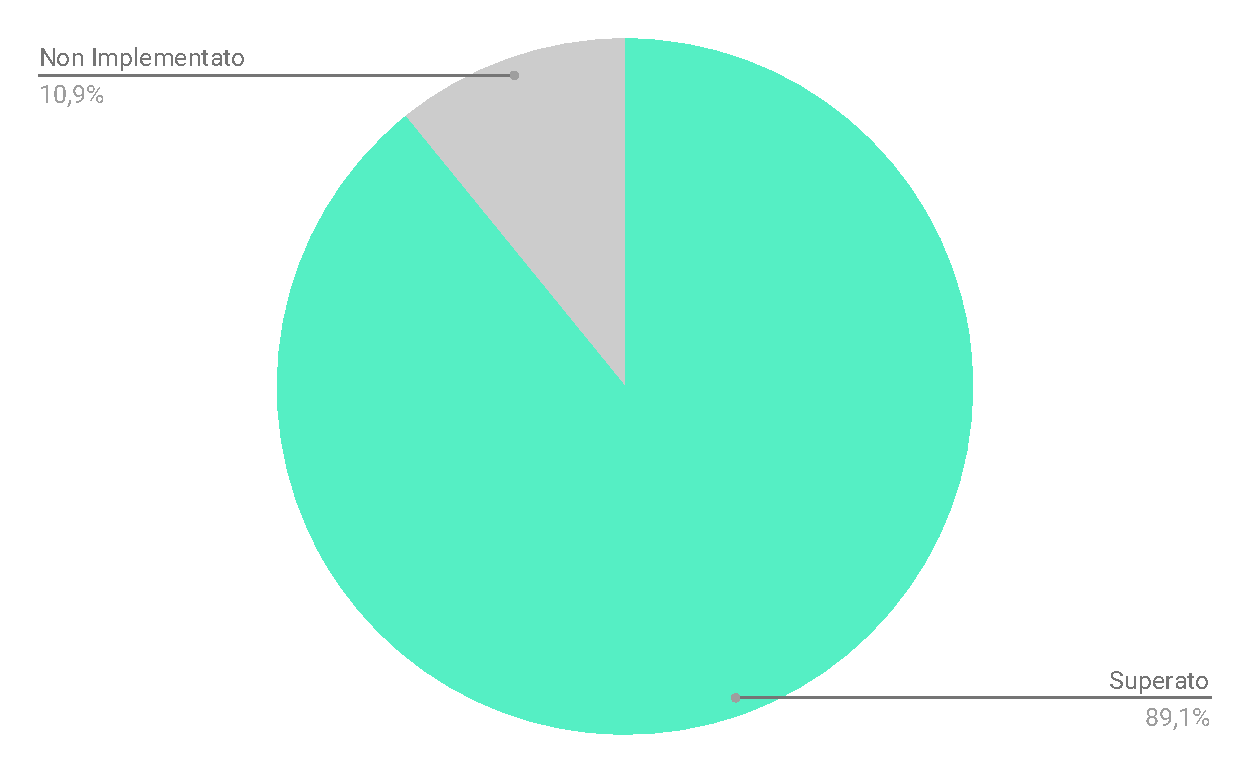
\includegraphics[width=0.7\linewidth]{sez/test/img/statoTestUnita.pdf}
% 	\caption{Riepilogo stato test di unità}
% \end{figure}

\subsubsection{Tracciamento Test di unità - Metodi}

\begin{tabularx}{\textwidth}{cX}
	
	\rowcolor{greySWEight}
	
	\rowcolor{greySWEight}
	\textcolor{white}{\textbf{Test}} & 
	\textcolor{white}{\textbf{Metodi}} \\
	
	TU001 & colletta::repository::user::UsersRepositoryImpl::updateActivateFlagOnly() \\
	TU002 & colletta::repository::user::UsersRepositoryImpl::getAllUsers() \\
	TU003 & colletta::repository::phrase::PhraseRepositoryImpl::findAllByAuthor() \\
	TU004 & colletta::repository::phrase::PhraseRepositoryImpl::findAllSolutionsByAuthor() \\
	TU005 & colletta::repository::phrase::PhraseRepositoryImpl::increaseReliability() \\
	TU006 & colletta::repository::phrase::PhraseRepositoryImpl::getSolution() \\
	TU007 & colletta::repository::exercise::ExerciseRepositoryImpl::modifyAuthorName() \\
	TU008 & colletta::service::user::UserService::addUser() \\
	TU009 & colletta::service::user::UserService::findById() \\
	TU010 & colletta::service::user::UserService::getUserInfo() \\
	TU011 & colletta::service::user::UserService::activateUser() \\
	TU012 & colletta::service::user::UserService::deleteUser() \\
	TU013 & colletta::service::user::UserService::findByEmail() \\
	TU014 & colletta::service::user::UserService::updateUser() \\
	TU015 & colletta::service::user::UserService::addExerciseItem() \\
	TU016 & colletta::service::user::UserService::findAllExerciseToDo() \\
	TU017 & colletta::service::user::UserService::getAllStudents() \\
	TU018 & colletta::service::user::UserService::getAllUsers() \\
	TU019 & colletta::service::user::UserService::removeAssignedExercise() \\
	TU020 & colletta::service::user::UserService::getAllExerciseDone() \\
	TU021 & colletta::service::user::UserService::addCompletedExercise() \\
	TU022 & colletta::service::user::UserService::getAllDevelopersToEnable() \\
	TU023 & colletta::service::SolutionService::getAutomaticCorrection() \\
	TU024 & colletta::service::PhraseService::insertPhrase() \\
	TU025 & colletta::service::PhraseService::getPhraseById() \\
	TU026 & colletta::service::PhraseService::increaseReliability() \\
	TU027 & colletta::service::PhraseService::getSolutionInPhrase() \\
	TU028 & colletta::service::ExerciseService::modifyExerciseAuthorName() \\
	TU029 & colletta::service::ExerciseService::insertExercise() \\
	TU030 & colletta::service::ExerciseService::doExercise() \\
	TU031 & colletta::service::ExerciseService::correct() \\
	TU032 & colletta::service::ExerciseService::deleteExercise() \\
	TU033 & colletta::service::ExerciseService::getAllByIds() \\
	TU034 & colletta::controller::Controller::deleteUser() \\
	TU035 & colletta::controller::Controller::getAllDevelopersToEnable() \\
	TU036 & colletta::controller::Controller::getAllUser() \\
	TU037 & colletta::controller::Controller::signUp() \\
	TU038 & colletta::controller::Controller::getUserInfo() \\
	TU039 & colletta::controller::Controller::modifyExerciseAuthorName() \\
	TU040 & colletta::controller::Controller::activateUser() \\
	TU041 & colletta::controller::Controller::insertExercise() \\
	TU042 & colletta::controller::Controller::doExercise() \\
	TU043 & colletta::controller::Controller::getAutomaticCorrection() \\
	TU044 & colletta::controller::Controller::getUserExercise() \\
	TU045 & colletta::controller::Controller::getExerciseDone() \\
	TU046 & colletta::controller::Controller::getStudentsList() \\
	% TU047 &	src::view::components::sidebarElementStudent() \\
	% TU048 & src::view::components::sidebarElementTeacher() \\
	% TU049 & src::view::components::sidebarElementAdministrator() \\
	% TU050 & src::view::components::sidebarElementDevelopment() \\
	% TU051 & 
	% TU052 & src::helpers::_translator() \\
	% TU053 & src::view::component::executionExercise() \\
	% TU054 & src::helper::SolutionMapper::getCodeSolution() \\
	% TU055 & src::helper::SolutionMapper::getVerboseSolution() \\
	% TU056 & src::helper::SolutionMapper::getSolution() \\
	% TU057 & src::helper::SolutionMapper::getCodeSolution() \\
	% TU058 & src::helpers::_translator() 
	% TU059 &
	% TU060 &
	% TU061 &
	% TU062 &
	% TU063 &
	% TU064 &
	% TU065 &
	% TU066 &
	% TU067 &
	% TU068 &
	% TU069 &
	% TU070 &
	% TU071 &
	% TU072 &
	% TU073 &
	% TU074 &
	% TU075 &
	% TU076 &
	% TU077 &
	% TU078 &
	% TU079 &
	% TU080 &
	% TU081 &
	% TU082 &
	% TU083 &
	% TU084 &
	% TU085 &
	% TU086 &
	\rowcolor{white}
	\caption{Tracciamento test di unità - metodi}
	\label{tab:tracciamentotestunità}
\end{tabularx}
